%%%%%%%%%%%%%%%%%%%%%%%%%%%%%%%%%%%%%%%%%%%%%%%%%%%%%%
\documentclass[12pt,a4paper]{report}
% o article, book, ...



%%%%%%%%%%%%%%%%%%%%%%%%%%%%%%%%%%%%%%%%%%%%%%%%%%%%%%
% packages...
\usepackage[utf8]{inputenc}
\usepackage[english,italian]{babel}
\usepackage[hyphens]{url}

% Per generare il file PDF aderente alle specifiche PDF/A-1b. Verificarne poi la validità.
%\usepackage[a-1b]{pdfx}

\usepackage{hyperref}
\usepackage{refcheck}
\usepackage{graphicx}
\graphicspath{{./img/}}

\usepackage{underscore} % !!!
\usepackage{hyperref}
%\usepackage{bera}% optional: just to have a nice mono-spaced font
\usepackage{listings}
\usepackage{xcolor}

\colorlet{punct}{red!60!black}
\definecolor{background}{HTML}{EEEEEE}
\definecolor{delim}{RGB}{20,105,176}
\colorlet{numb}{magenta!60!black}

\lstdefinelanguage{json}{
    basicstyle=\normalfont\ttfamily,
    numbers=left,
    numberstyle=\scriptsize,
    stepnumber=1,
    numbersep=8pt,
    showstringspaces=false,
    breaklines=true,
    frame=lines,
    backgroundcolor=\color{background},
    literate=
     *{0}{{{\color{numb}0}}}{1}
      {1}{{{\color{numb}1}}}{1}
      {2}{{{\color{numb}2}}}{1}
      {3}{{{\color{numb}3}}}{1}
      {4}{{{\color{numb}4}}}{1}
      {5}{{{\color{numb}5}}}{1}
      {6}{{{\color{numb}6}}}{1}
      {7}{{{\color{numb}7}}}{1}
      {8}{{{\color{numb}8}}}{1}
      {9}{{{\color{numb}9}}}{1}
      {:}{{{\color{punct}{:}}}}{1}
      {,}{{{\color{punct}{,}}}}{1}
      {\{}{{{\color{delim}{\{}}}}{1}
      {\}}{{{\color{delim}{\}}}}}{1}
      {[}{{{\color{delim}{[}}}}{1}
      {]}{{{\color{delim}{]}}}}{1},
}


% Per inserire testo a caso in attesa di realizzare i capitoli
%\usepackage{lipsum}

\usepackage{todonotes}
%\usepackage[disable]{todonotes} % alla fine mettere

\usepackage[a4paper,top=2cm,bottom=2cm,outer=5cm,verbose,headheight=1cm,heightrounded]{geometry}
\setlength{\marginparwidth}{4.5cm} %per farci stare todonotes, nel final si può rimuovere



%%%%%%%%%%%%%%%%%%%%%%%%%%%%%%%%%%%%%%%%%%%%%%%%%%%%%
\begin{document}

% Frontespizio
\begin{titlepage}
  \begin{center}
    
\includegraphics[width=\textwidth]{Logo.jpg}\\
    {\large{\bf Corso di Laurea in Informatica}}
  \end{center}
  \vspace{12mm}
  \begin{center}
    {\huge{\bf CONVERSIONE DI}}\\
    \vspace{4mm}
    {\huge{\bf STRUMENTI VINTAGE}}\\
    \vspace{4mm}
    {\huge{\bf PER LA DATA}}\\
    \vspace{4mm}
    {\huge{\bf PHYSICALIZATION}}\\
  \end{center}
  \vspace{12mm}
  \begin{flushleft}
    {\large{\bf Relatore:}}
    {\large{Andrea Trentini}}\\
    %\vspace{4mm}
    %{\large{\bf Correlatore:}}
    %{\large{...}}\\
  \end{flushleft}
  \vspace{12mm}
  \begin{flushright}
    {\large{\bf Tesi di Laurea di:}}
    {\large{Davide Busolin}}\\
    {\large{\bf Matr. 930814}}\\
  \end{flushright}
  \vspace{4mm}
  \begin{center}
    {\large{\bf Anno Accademico 2020/2021}}
  \end{center}
\end{titlepage}

\listoftodos
\tableofcontents


% REPORT
%\part
%	\chapter
%		\section
%			\subsection
%				\paragraph
%					\subparagraph

% o sections (dipende dal documentclass)
\chapter{Introduzione}
\section{Data Physicalization: definizione}
Una data physicalization (in italiano: fisicalizzazione dei dati) è un artefatto fisico la cui geometria o proprietà materiali codificano dei dati.\cite{dataphysorg:terminology}
\todo{atrent: in generale i link web li metterei in footnote, se vuoi lasciarli in bib devi mostrare anche l'url}
\todo{atrent: puoi eliminare tutti i doppi backslash, non servono}
Gli stessi autori della precedente definizione distinguono tra data physicalization come artefatti (per i quali vale quanto scritto sopra),
data physicalization come il processo di dare forma fisica ai dati e data physicalization come l'area di ricerca che unisce da visualizzazione
dei dati e interfacce utenti tangibili.

\section{Visualizzazione dei dati}
Lo scopo della disciplina della visualizzazione dei dati è quello di renderli più comprensibili per gli esseri umani. I display dei computer
sono l'esempio più classico, hanno molti vantaggi grazie alla loro versatilità tra cui di fornire rappresentazioni visuali dei dati in
maniera dettagliata e modificabile dinamicamente. Tuttavia, è emersa un'area di ricerca che pone la questione di non limitarsi a una
matrice di pixel per visualizzazione di e interazione con i dati ma sfruttare altri tipi di interazione più naturale per gli esseri umani, come
è stato dimostrato dalla ricerca in Tangible Computing. \cite{hal:dataphys} \\
\todo{atrent: in generale van riportati i principali concetti esposti negli articoli/libri che citi}

\section{Esempi di data physicalization e visualization}
\todo{atrent: fai anche esempi non miei, prendi quelli che ti piacciono di più, due o tre esempi}

\subsection{Keyboard Frequency Sculpture}
Un diagramma a barre 3D appoggiato su una tastiera che mostra la frequenza di ciascuna lettera dell'alfabeto. \cite{physlist}, Figura~\ref{fig:keyboardfreq}
\begin{figure}[h]
  \centering
  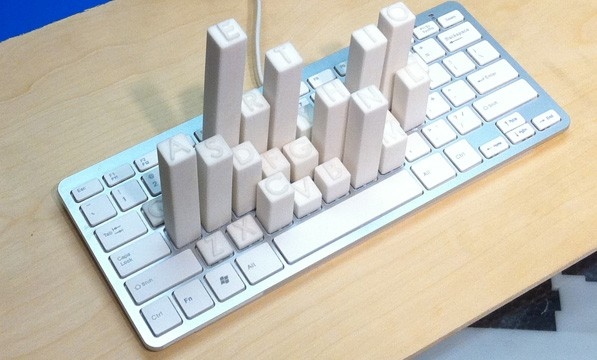
\includegraphics[width=0.6\textwidth]{keyboardfreq}
  \caption{Keyboard Frequency Sculpture}
  \label{fig:keyboardfreq}
\end{figure}

\subsection{Living Map: Precipitation Visualized with Moss}
Mappa "vivente" che mostra il cambiamento nella quantità di precipitazioni nelle varie zone d'Europa a seguito del riscaldamento climatico
mediante l'erogazione controllata di acqua su un particolare tipo di muschio.  \cite{physlist}, Figura~\ref{fig:livingmap}
\begin{figure}[h]
  \centering
  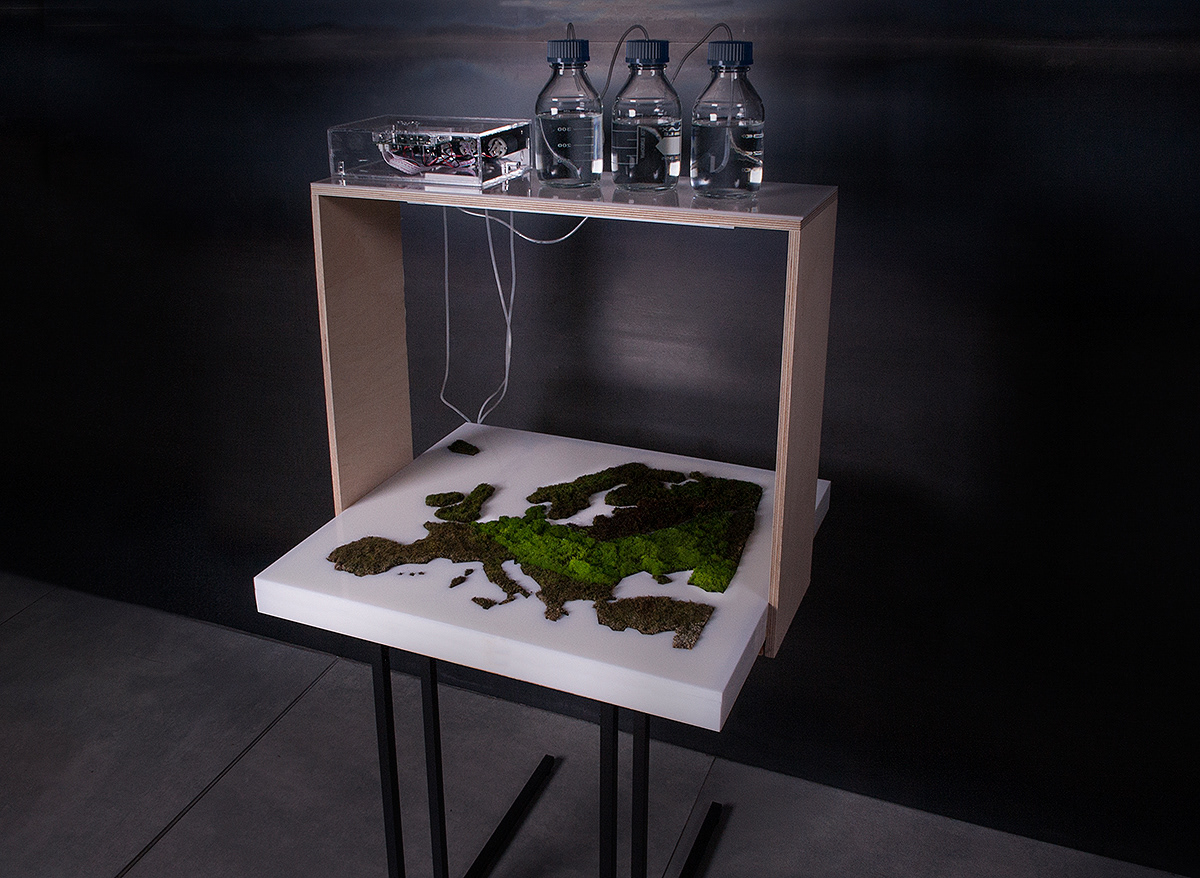
\includegraphics[width=0.8\textwidth]{livingmap}
  \caption{Living Map: Precipitation Visualized with Moss}
  \label{fig:livingmap}
\end{figure}

% Altra papabile: http://dataphys.org/list/self-knitted-scarf-of-train-delays/

\subsection{Physiradio}
Una radio vintage che riproduce musica di mood/genere correlato alle condizioni metereologiche. Figura~\ref{fig:physiradio}
\begin{figure}[h]
  \centering
  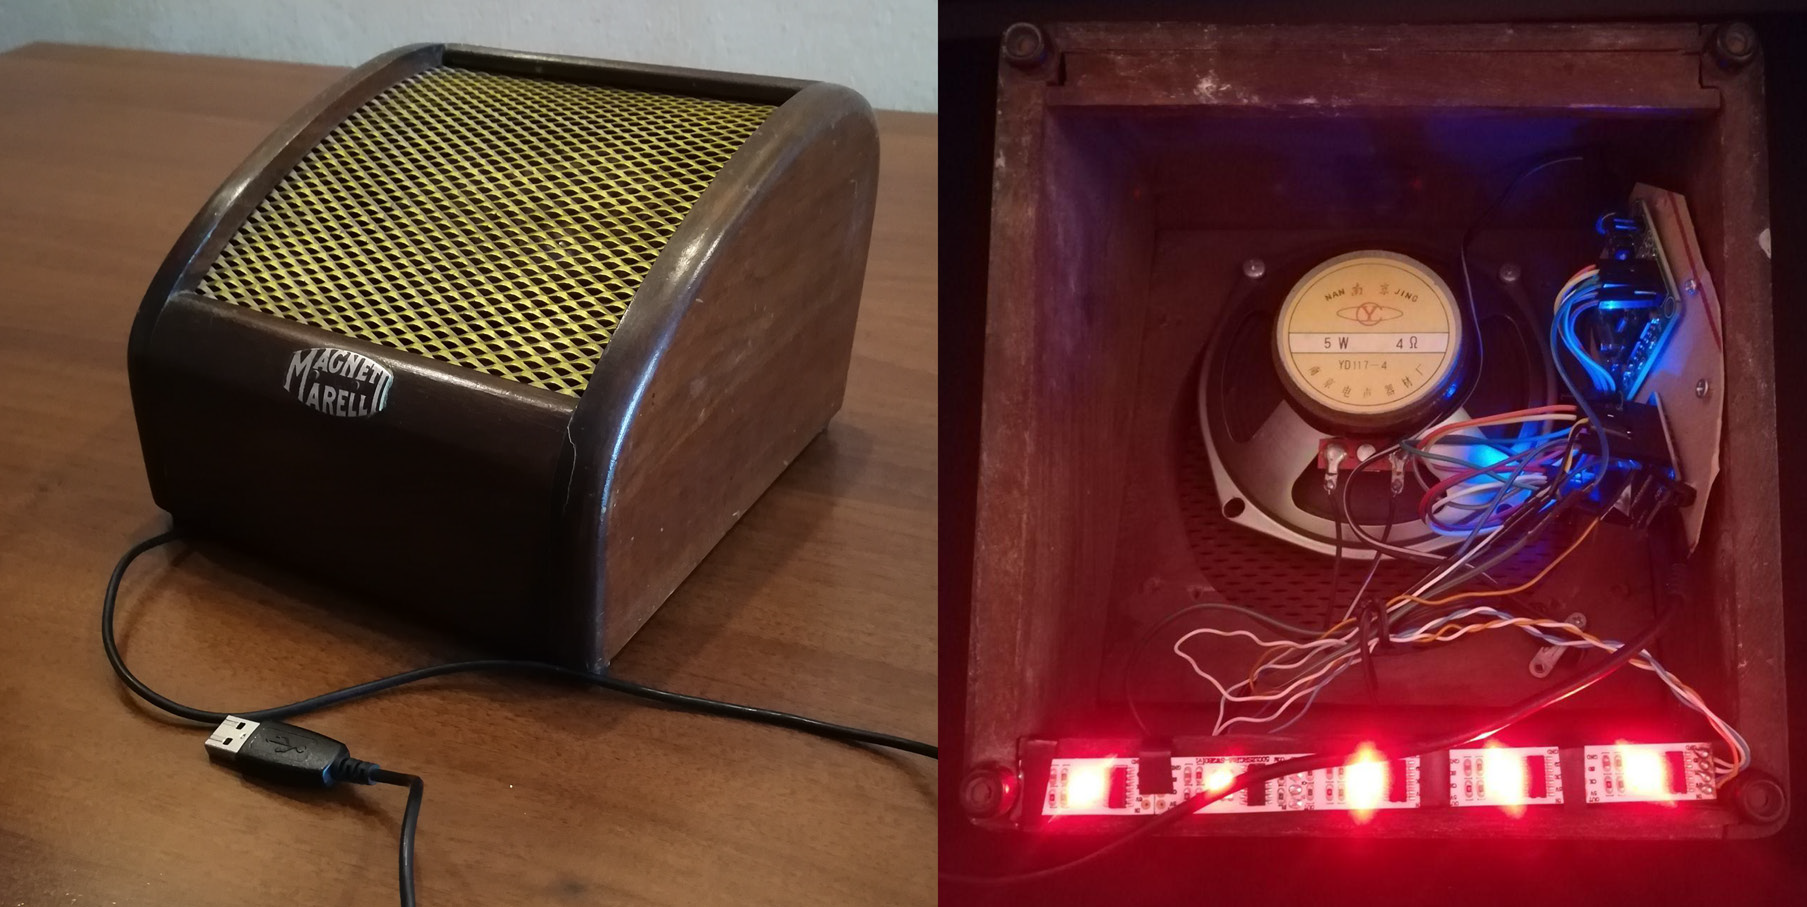
\includegraphics[width=0.8\textwidth]{physiradio}
  \caption{Physiradio \cite{physiradio}}
  \label{fig:physiradio}
\end{figure}

\subsection{BiblioVisualizer}
Visualizzazione dei dati sul prestito libri nel consorzio Culture Socialità Biblioteche Network Operativo (CSBNO) tramite barra di LED.
\cite{bibliovisgitlab}, Figura~\ref{fig:bibliovisualizer}
\begin{figure}[h]
  \centering
  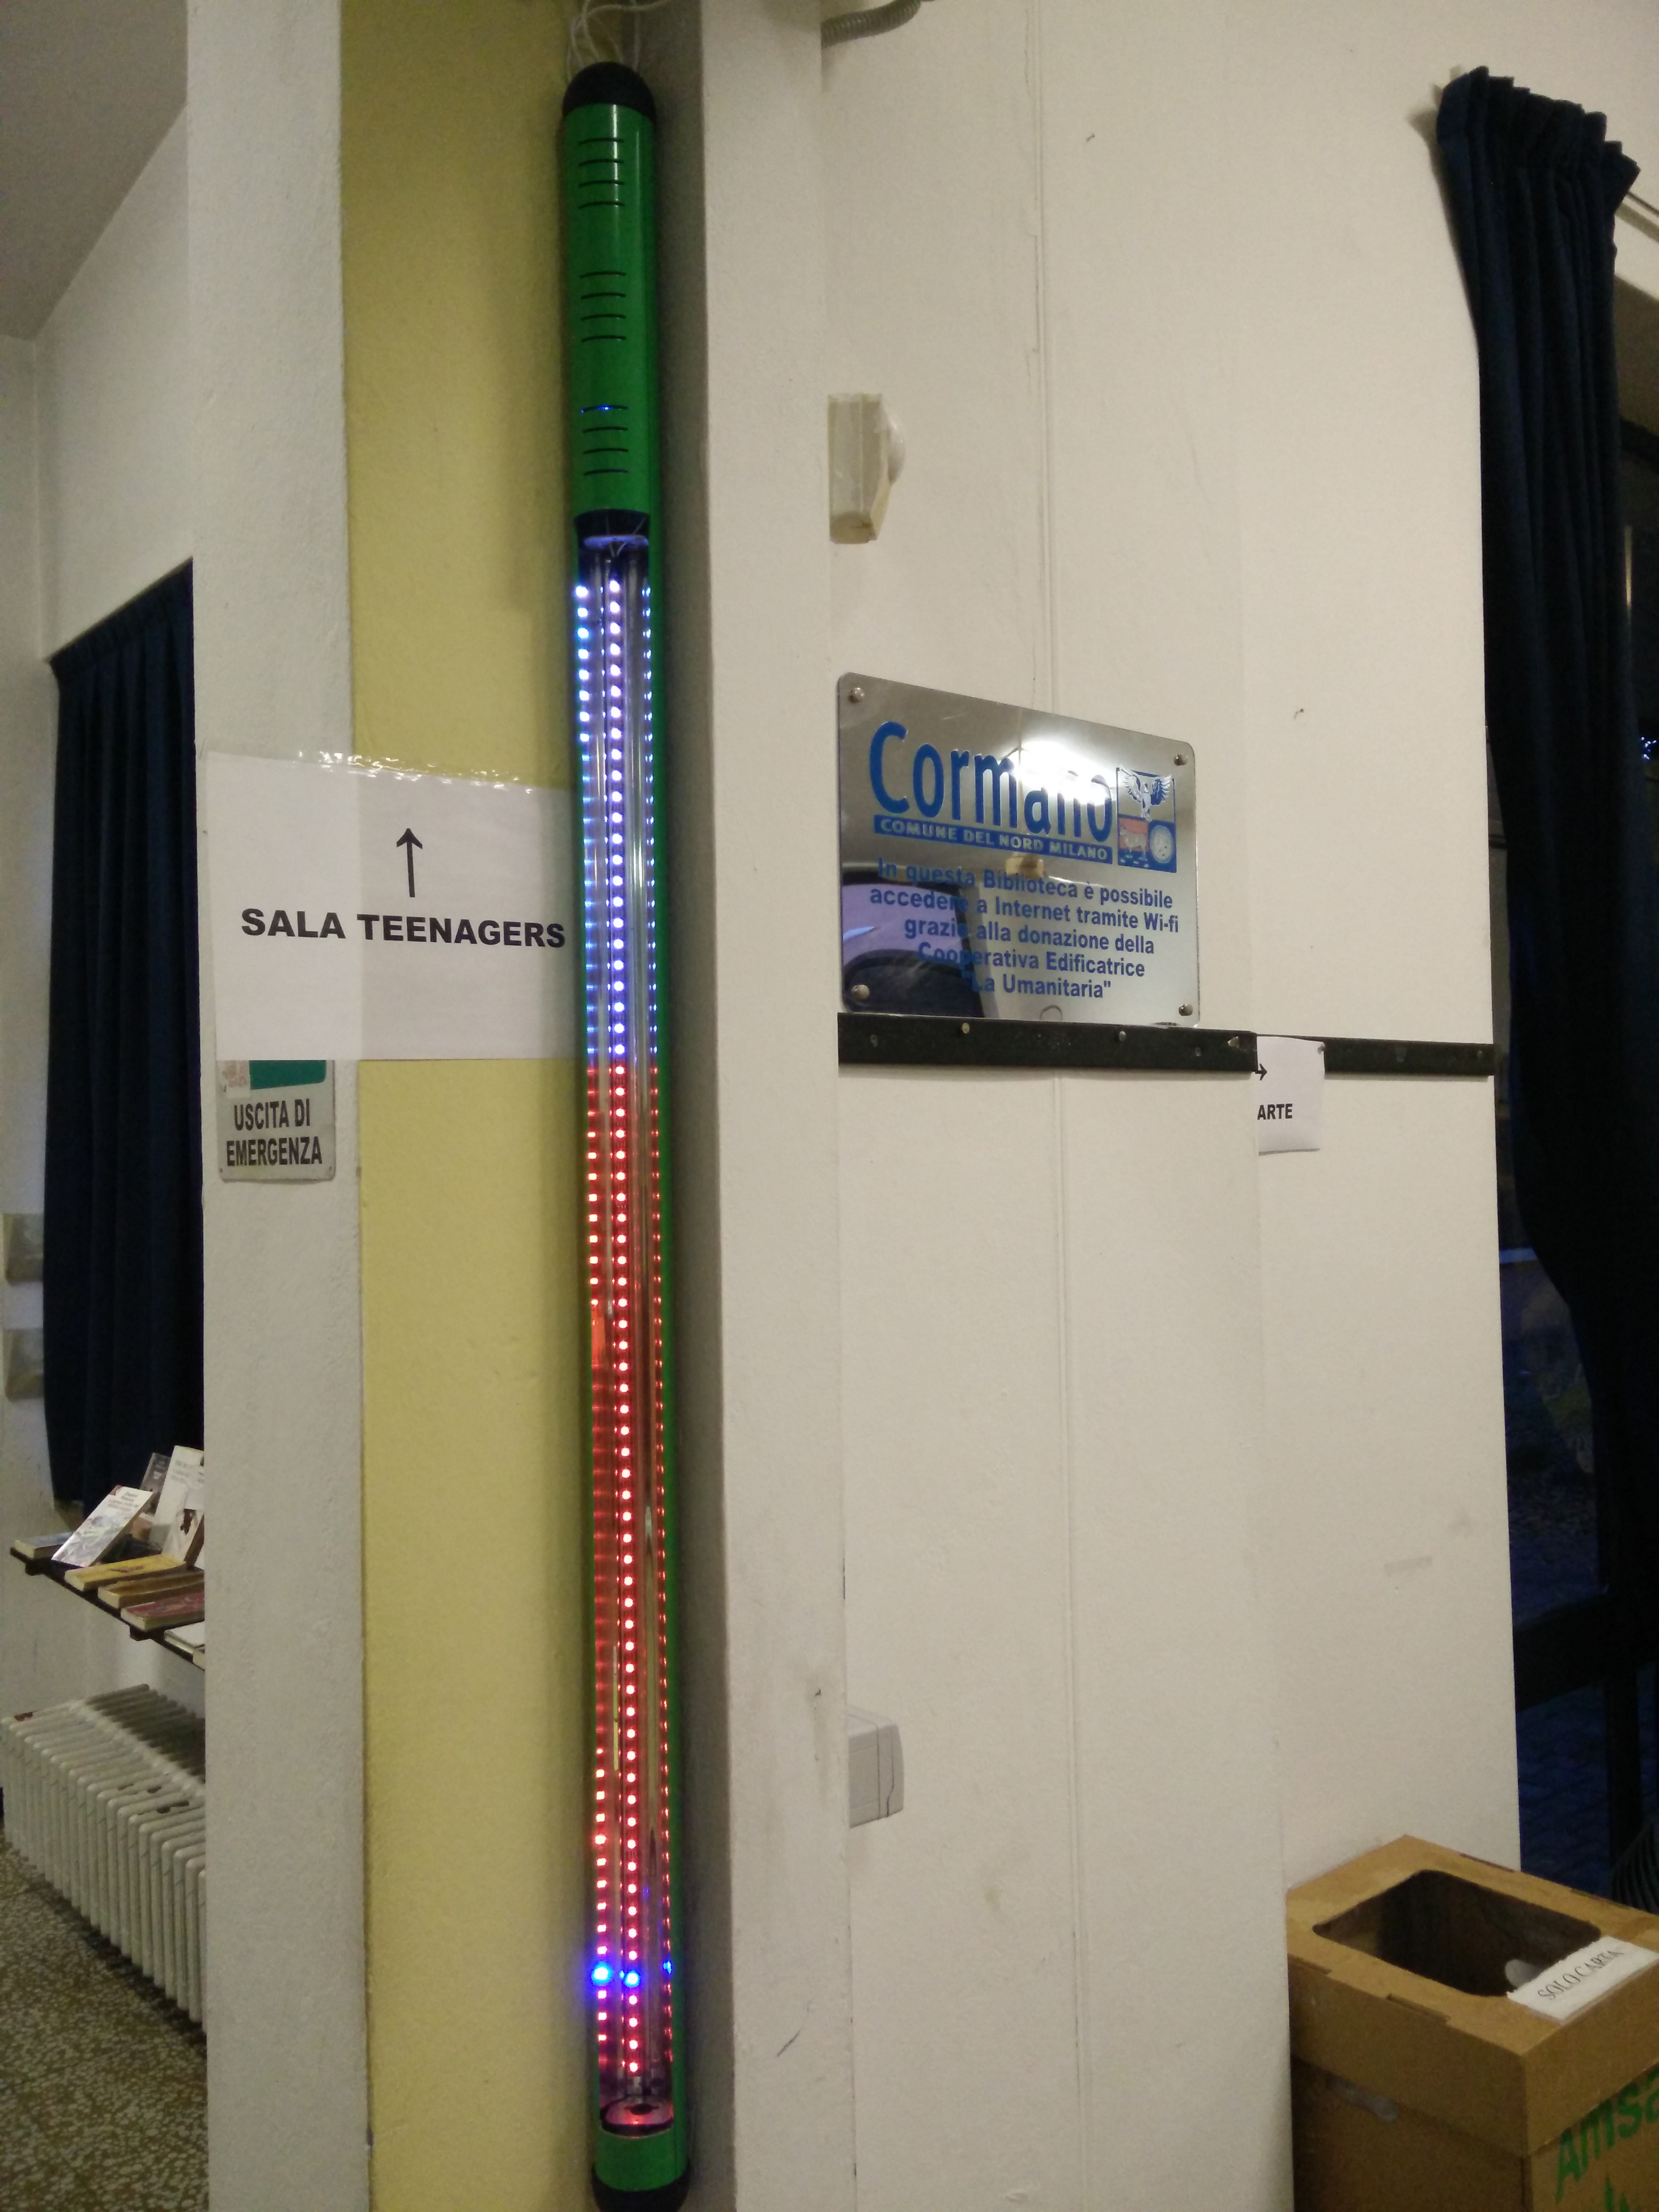
\includegraphics[width=0.5\textwidth]{bibliovisualizer}
  \caption{BiblioVisualizer}
  \label{fig:bibliovisualizer}
\end{figure}


%%%% Sezione IoT?

\section{Obiettivo}
L'obiettivo dell'attività svolta durante il tirocinio è quello di analizzare e sperimentare una forma di fisicalizzazione
dei dati mediante strumenti di misura vintage e dispositivi IoT che non richieda l'utilizzo di computer e monitor e sia di semplice fruizione
da parte di chi non è avvezzo alla tecnologia e può essere intimorito da complicate dashboard o semplicemente privo della volontà
di interagire con dispositivi tecnologici per l'ottenimento di certe informazioni. L'utilizzo di strumenti vintage consente infatti di ottenere
oggetti discreti che possono far parte dell'arredamento domestico, ad esempio su una mensola, i quali invece di essere puramente
decorativi comunicano informazioni utili.

% Tecnofobia
% Esempi dashboard?


\chapter{Generalizzazione degli strumenti di misura}
In questo capitolo si tenterà di generalizzare le caratteristiche degli strumenti di misura ai fini di associarle a componenti software e tipi di dato.
\todo{atrent: strada giusta! fai anche esempi pratici finali}
\section{Indicatori}
\subsection{Strumenti ad ago}
Sono il tipo più comune di strumenti di misura vintage. Un esempio sono i voltmetri / amperometri / multimetri analogici che si utilizzavano
fino a pochi anni fa. Possono essere utilizzati per visualizzare grandezze lineari, facendo attenzione alla scala scelta.

\section{Interazione con l'utente}

\subsection{Interruttori}
Possono essere mappati a valori booleani (true/false)

\subsection{Commutatori a n posizioni}
Possono essere mappati in un programma a tipi \texttt{enum}, utilizzabili per selezionare tra un insieme di modalità o un insieme di valori
utilizzabili come parametro in un programma. Ad esempio un commutatore a 7 posti può essere utilizzato per selezionare un giorno della
settimana.

\subsection{Potenziometri}
Consentono di variare una differenza di potenziale nel continuo quindi possono essere mappati a valori aventi intervallo arbitrario, con una precisione limitata dalla risoluzione del convertitore analogico-digitale integrato nel microcontrollore.

\subsection{Connettori multipli}
Alcuni strumenti dispongono di più ingressi per le sonde di misura, adatti a connettori a banana o non standard, e specifici alle
diverse modalità di misura e/o i diversi fondoscala tra cui scegliere. Possono essere utilizzati come selettori a livello software in base a
quali degli ingressi vengono ponticellati, in maniera simile alle connessioni tra utenze telefoniche nei vecchi centralini o agli spinotti per
gli scambi di lettere presenti sulla macchina Enigma.



\chapter{Guida alla trasformazione degli strumenti vintage}

\todo{atrent: manca una trattazione di come è fatto e come funziona lo strumento ad ago (che sarà il più frequente oggetto di visualizzazione), spiega bene la sua architettura, wikipedia is your friend}


\todo{atrent: tenterei anche una panoramica storica degli strumenti di ``visualizzazione'' (occhi magici, elettrofori, dekatron, oscilloscopi, ...) dando idee su come si potrebbero usare per datafisicalizzare}


Una volta appurate le caratteristiche degli strumenti, è opportuno discutere degli interventi fisici necessari alla loro conversione.


Il metodo più semplice per ottenere un oggetto funzionante è quello di collegare il GPIO del microcontrollore settato come output
e GND rispettivamente al terminale positivo e negativo dello strumento di misura in modalità voltmetro. Se la tensione in uscita massima
coincide con il fondoscala dello strumento di misura questo è sufficiente, altrimenti è necessario ridurla via software oppure
utilizzare un partitore di tensione o un potenziometro. Nel caso in cui la tensione in uscita massima del microcontrollore sia inferiore
ad ogni possibile fondoscala dello strumento di misura, questo metodo non è attuabile.

Un metodo più invasivo ma più pulito consiste nel modificare la struttura interna dello strumento di misura, collegandosi ai capi dello
strumento interno vero e proprio bypassando selettore di modalità/fondoscala.
Se non si vuole rimpiazzare la resistenza interna valgono le stesse osservazioni fatte poc'anzi sui fondoscala: è necessario che
esista una modalità con fondoscala minore o uguale alla tensione di uscita massima del microcontrollore, altrimenti sarà necessario
utilizzare una resistenza più piccola di quella/e già presente/i. \\
Questa operazione consente di integrare (a condizione che ci sia spazio) il microcontrollore all'interno dello strumento in modo da
ottenere un sistema composto da un solo oggetto. Se si ha la facoltà di inserire una batteria diventa anche incredibilmente discreto
e di più facile posizionamento, anche dove è scomodo portare una fonte di alimentazione.

Ulteriori possibili modifiche meno banali includono l'aggiunta di elementi decorativi quali delle luci o funzionali quali bottoni o altoparlanti
per ampliare le possibilità di utilizzo. Un'altra possibilità di modifica ove possibile è la sostituzione dell'etichetta sotto all'ago per adattare
la scala rappresentata alla vera scala dei dati (a condizione che questa rimanga fissa).


\chapter{Use case}
Prima di parlare del funzionamento dell'oggetto è il caso di soffermarsi su chi interagisce con esso e in che modo:  %%Rivedere frase
\subsection*{Sviluppatore}
È in grado di apportare modifiche al codice sorgente. Può aggiungere, rimuovere e  modificare funzionalità del programma
e apportare modifiche dirette ai file di configurazione.
\subsection*{Utente esperto}
Conosce le API ed è in grado di comprendere il formato dei dati che restituiscono. Gli è sufficiente un'interfaccia anche spartana
per selezionare la sorgente dei dati e il campo specifico che vuole rappresentato.
\subsection*{Utente inesperto}
Non conosce le API né il formato JSON: ha bisogno di un prodotto già pronto che richieda la minima configurazione possibile e questa
deve essere particolarmente intuitiva, ad esempio una piccola interfaccia web per scegliere la rete WiFi e inserirne la password
al primo avvio. La sorgente dei dati deve essere preconfigurata e se ne viene resa disponibile più di una la scelta deve essere molto
semplice, possibilmente tramite interazione fisica con il dispositivo.

\todo{atrent: questi sono i ruoli, mancano gli use case veri e propri (parlando formalmente, faccio riferimento a UML)}

\todo{atrent: in generale metterei tanti schemi e disegni}

\chapter{Utilizzo del prototipo}

\section{All'avvio}
Per prima cosa contestualmente all'accensione, mediante WiFiManager, viene effettuato un tentativo di connessione all'ultima rete WiFi
utilizzata, di cui sono state salvate le credenziali. Se non è mai stata effettuata la connessione ad alcuna rete WiFi o se
quella salvata non è disponibile, viene attivato un Access Point che tramite Captive Portal (lo stesso che viene usato su reti pubbliche
o aziendali per richiedere l'autenticazione) chiede di selezionare una delle reti WiFi vicine e di inserirne la password.\\

\vspace{4mm}
{[SCREENSHOT]}\\
\vspace{4mm}

Successivamente viene tentata la connessione. Se non ha successo viene riproposto lo stesso procedimento, altrimenti viene disattivato
l'Access Point temporaneo e il programma prosegue.

\pagebreak
\section{Modalità operative}

\subsection{Modalità API}
Questa modalità di operazione si basa sull'esecuzione ad intervalli di tempo configurabili di richieste HTTP o HTTPS ad API REST
e sulla conversione del risultato in una tensione di uscita.
La configurazione è salvata nella memoria flash del microcontrollore
in formato JSON, esempio:

\begin{lstlisting}[language=json,firstnumber=1]
{
  "apiUrl": "http://api.coindesk.com/v1/bpi/currentprice/USD.json",
  "filterJSON": "{bpi:{USD:{rate_float:true}}}",
  "path": "bpi/USD/rate_float",
  "min_value": 58700,
  "max_value": 58900,
  "min_pwm": 0,
  "max_pwm": 1023,
  "request_interval_ms": 15000
}
\end{lstlisting}


\noindent Dove:
\begin{itemize}
  \item \texttt{apiUrl} è l'URL della risorsa (stringa)
  \item \texttt{post_payload} in caso di richiesta POST contiene la stringa da inviare nel body
  \item \texttt{filterJSON} è un documento JSON che contiene \texttt{true} come placeholder del campo che si vuole considerare dalla risposta (stringa/oggetto)
  \item \texttt{path} è una stringa che contiene il "percorso" del campo che si vuole rappresentare fisicamente (campo: float, path: stringa)
  \item \texttt{min_value} indica il valore minimo della scala per rappresentare il valore (float)
  \item \texttt{max_value} indica il valore massimo (float)
  \item \texttt{min_pwm} indica il valore minimo di uscita della PWM da mappare al valore restituito dalle API (int)
  \item \texttt{max_pwm} indica il valore massimo [su ESP il duty cycle massimo equivale a 1023] (int)
  \item \texttt{request_interval_ms} indica l'intervallo di tempo in millisecondi che intercorre tra le richieste alla risorsa (int)
\end{itemize}

La configurazione può essere alterata tramite una pagina web accessibile all'indirizzo IP nella rete locale del microcontrollore o il suo
hostname.

\vspace{4mm}
{[SCREENSHOT PAGINA WEB]}

\vspace{4mm}
I form sono precompilati con la configurazione in esecuzione (\emph{running-conf}) ed è presente una sezione che riporta la configurazione
salvata nella flash (\emph{saved-conf}).\\
È possibile inoltre inviare un JSON di configurazione tramite MQTT al topic \texttt{Phys/setFromJSON}. I campi possono essere modificati
singolarmente ai topic:
\begin{itemize}
  \item \texttt{Phys/setApiUrl}
        % ToDo: setPostPayload
  \item \texttt{Phys/setFilterJson}
  \item \texttt{Phys/setPath}
  \item \texttt{Phys/setMinValue}
  \item \texttt{Phys/setMaxValue}
  \item \texttt{Phys/setMinPwm}
  \item \texttt{Phys/setMaxPwm}
  \item \texttt{Phys/setRequestIntervalMs}
\end{itemize}

Le modifiche non sono automaticamente salvate nella memoria flash ma ciò deve essere richiesto esplicitamente. Nei form di configurazione
è presente una checkbox da spuntare in caso si voglia che questo avvenga.


\subsection{Modalità MQTT}
Non ancora implementata, ma l'idea è che consenta di visualizzare un valore ricevuto direttamente tramite sottoscrizione a un topic MQTT
invece che andarlo a reperire tramite richieste HTTP(S).

\chapter{Realizzazione del prototipo}

\section{Hardware}
Il prototipo è molto semplice dal punto di vista hardware, consiste in un voltmetro analogico ad ago e un WeMos D1 mini basato su ESP8266.\\
Il terminale positivo del voltmetro è connesso a un GPIO dell'ESP, mentre il terminale negativo a terra. È configurato mediante i
commutatori in modalità corrente continua con fondo scala a 3V.

\section{Software}
La parte software del prototipo è stata realizzata utilizzando il linguaggio di programmazione di Arduino, esteso all'utilizzo con
ESP8266 e con l'aiuto di numerose librerie.

\subsection{PWM}
Il principio di base che permette di produrre una tensione variabile da parte di un sistema digitale è la Pulse-Width Modulation.\\
Ciò permette di controllare finemente la posizione dell'ago del voltmetro via software.

\subsection{Richieste API}
Il primo passo verso la fisicalizzazione dei dati è stato quello di ottenerli, mediante richieste ad API REST in locale o su Internet.
Per questo è stata utilizzata la libreria \texttt{ESP8266HTTPClient}.\\
Le richieste HTTP hanno funzionato fin da subito, per HTTPS c'è stato più da lavorare in quanto non erano eccessivamente
documentate e tutte le soluzioni trovate online prevedevano l'utilizzo di stringhe per memorizzare intere risposte, che per via
della limitata disponibilità di memoria dell'ESP non è sempre una soluzione funzionante.\\
Un'alternativa fornita dalla libreria è quella di utilizzo di uno stream, per poter leggere dalla risposta un byte alla volta senza doverla
memorizzare per intero, potendo ignorare le parti non necessarie. Questo meccanismo però è di facile utilizzo solo finché ci si limita a
HTTP. Per HTTPS la funzione per estrarre lo stream della risposta, secondo la documentazione della libreria, non è supportata.
Come soluzione è stato utilizzato come stream direttamente il BearSSL::WiFiClientSecure referenziato dalla connessione, impostato in
modalità insicura (senza la verifica della fingerprint), che però non sempre presenta un output "pulito" della risposta ma potrebbe essere
preceduto da una linea contentente (presumibilmente) la lunghezza in byte della risposta.

\subsection{JSON}
La quasi totalità delle API mette a disposizione risposte contenenti dati in formato JSON (JavaScript Object Notation), è stata quindi
utilizzata la libreria \texttt{ArduinoJson} per la deserializzazione e la scelta del campo da estrarre.\\
JSON è stato successivamente usato anche come formato per la serializzazione e deserializzazione delle impostazioni da salvare sulla
memoria flash dell'ESP per permetterne la persistenza anche a seguito di perdite di tensione.

\subsection{Approfondimento su filtro JSON e path} %Giusto averlo qui o meglio in sezione a parte?
Il centro del funzionamento della modalità API e la sua adattabilità all'utilizzo di fonti dati diverse risiede nei campi
filterJSON e path.\\
\texttt{filterJSON} consente di evitare che tutta la risposta delle API venga salvata in memoria. Viene quindi scartato ogni campo che non
appaia come placeholder all'interno della stringa, ad esempio:\\
\texttt{"\{Lines: [\{WaitMessage: true\}]\}"} consente di mantenere
in memoria solo il campo con chiave WaitMessage di ogni elemento contenuto nell'array avente chiave Lines. Questa funzionalità è
implementata e ben documentata nella libreria \texttt{ArduinoJSON}.~\cite{arduinojsonfiltering} \\
Questo filtro non è sufficiente come indicatore del campo desiderato, in quanto il documento JSON salvato in memoria conterrà comunque
tutta la gerarchia e per come funzionano i placeholder sugli array non è neanche detto che ci sia in totale un solo campo con un valore
assegnato.\\
Per questo motivo è stato aggiunto il campo \texttt{path} alla configurazione. Questa stringa, nel programma, viene interpretata token per
token usando lo slash come separatore e usata per esplorare la gerarchia dei campi. Un token completamente numerico viene visto come
indice di un array, altrimenti come chiave da cercare all'interno di un oggetto.\\
Per fare un esempio coerente con il precedente: \texttt{"Lines/0/WaitMessage"} verrà approcciato nel seguente modo:
\begin{itemize}
  \item Interpretare la radice come un oggetto, cercare la chiave \texttt{Lines} e spostarvisi all'interno;
  \item Interpretare il successivo livello come un array, estrarre l'elemento in posizione 0 e spostarvisi all'interno;
  \item Interpretare il successivo livello come un oggetto, cercare la chiave \texttt{WaitMessage} e spostarvisi all'interno.
\end{itemize}
A questo punto, finita la stringa, il programma assumerà di trovarsi dinnanzi a un campo interpretabile come numerico (tollera molto,
ad esempio la stringa "123aaa" verrà interpretata come 123.00), lo estrarrà e lo rappresenterà in output.\\ %excursus JsonVariant?
Questo approccio grazie al modo in cui è implementata la libreria è molto tollerante a errori o inesattezze. Se nel JSON non fosse
presente il campo desiderato il parsing della path, così come la conversione da stringa a numero presente subito dopo, non causerebbero
alcun crash del programma. È quindi possibile avere filtro e path inizialmente non corretti e adattarli tramite trial and error senza
causare riavvii indesiderati del microcontrollore a seguito di eccezioni.

\subsection{Map}
Una volta ottenuto il valore da rappresentare è necessario trasformarlo in una tensione, ottenuta tramite PWM il cui duty cycle è
proporzionale a un numero a 10 bit (0 - 1023). Per fare questo è possibile utilizzare la funzione \texttt{map} già presente nella
libreria standard di Arduino.\\
Durante i test è emerso che tale funzione non si comporta particolarmente bene quando uno dei range è formato da piccoli numeri
decimali. Si è quindi preferito inserire nel codice direttamente la formula matematica su cui si basa \texttt{map}:
\[out = \frac{(value - fromLow) \times (toHigh - toLow)}{(fromHigh - fromLow)} + toLow \]

\noindent Dove:\cite{arduinomap}
\begin{itemize}
  \item value: Il numero da mappare.
  \item fromLow: Il limite inferiore dell'intervallo corrente del valore
  \item fromHigh: Il limite superiore dell'intervallo corrente del valore
  \item toLow: Il limite inferiore dell'intervallo di destinazione del valore
  \item toHigh: Il limite superiore dell'intervallo di destinazione del valore
\end{itemize}

\subsection{Task}
Attività periodiche come le richieste API sono state rese dei task per mezzo della libreria \texttt{TaskScheduler}, che permette di
impostare un intervallo di tempo tra esecuzioni ripetute di una procedura.

\subsection{Configurazione via MQTT}
Come prima modalità di modifica "a runtime" della configurazione, è stata implementata la possibilità di inviare messaggi MQTT ai
topic precedentemente descritti

\subsection{Credenziali WiFi}
Per la connessione alla rete wireless, grazie alla libreria \texttt{WiFiManager}, l'ESP memorizzerà le ultime credenziali utilizzate
per ritentare la connessione al riavvio. In caso le credenziali non siano valide o non ve ne siano di salvate, verrà avviato un
Access Point temporaneo con captive portal per richiedere delle credenziali valide.

\subsection{Configurazione tramite form web}
Un'altra forma di modifica della configurazione è stata implementata tramite un web server configurato per mezzo della libreria
\texttt{ESPAsyncWebServer}. Inizialmente la pagina conteneva un semplice form tramite il quale era possibile inviare un intero JSON
di configurazione, successivamente è stata aggiunta la possibilità di impostare i singoli parametri attraverso un form precompilato
e richieste AJAX. Un punto debole di questa soluzione è la scarsa flessibilità del web server, che gestisce richieste POST solo codificate
come Form Data, quindi invece che poter mandare un semplice JSON nel body della richiesta come da prassi con AJAX, è stato necessario
trasformarlo in FormData come valore associato alla chiave setFromJSON.\\
Nel dettaglio, sono esposti i seguenti endpoint:
\begin{itemize}
  \item /: Pagina di configurazione (index.html)
  \item /get/running-conf: Restituisce la configurazione attualmente in esecuzione in formato JSON
  \item /get/saved-conf: Restituisce il file di configurazione presente nella memoria flash
  \item /post: permette di inviare un intero JSON di configurazione (anche incompleto, vengono modificati solo i campi specificati) come
        valore associato alla chiave setFromJSON. È inoltre possibile asssociare alla chiave saveToFlash il valore `true' per copiare
        la configurazione in esecuzione nella memoria flash.
\end{itemize}
%%%%%% Da rivedere

\subsection{OTA}
Sono stati implementati gli aggiornamenti OTA (Over the Air), processo tramite il quale è possibile eseguire l'upload di firmware
mediante WiFi invece che tramite porta seriale. Questo rimuove l'obbligo di utilizzo di una connessione cablata ed è molto utile
in situazioni di difficile accesso fisico al microcontrollore.\\
Il processo di upload usa Digest-MD5 per la verifica dell'integrità, onde evitare di rendere il dispositivo inservibile. È inoltre possibile
migliorare la sicurezza dell'operazione mediante utilizzo di password e hash firmati. \cite{espota}


\chapter{Conclusioni}

\todo{atrent: oltre alla presentazione all'hacklab (domani!) proviamo a organizzare una sessione ad hoc almeno con gli studenti del corso SistEmbed (e magari quelli di PROS?)}

\section{Reperibilità delle API}
Durante la ricerca di API rappresentabili mediante Data Physicalization è risultato evidente che molte di quelle più congeniali non
sono pubbliche e spesso sono anche di difficile utilizzo. L'esperienza personale è stata con quelle di ATM per ottenere i minuti rimanenti
all'arrivo di un mezzo pubblico ma altri si sono scontrati con quelle di Trenitalia \cite{trenitaliashock}

\subsection{Dettagli su ATM}
Le API di ATM sono usate per \href{https://giromilano.atm.it}{Giromilano} e l'unico modo per comprenderne il funzionamento è utilizzare
gli strumenti del browser per leggere le richieste e le risposte che vengono scambiate tra client e server durante la ricerca di un
percorso o di informazioni su una fermata specifica.\\
In particolare per ottenere i minuti rimanenti all'arrivo di un mezzo ad una specifica fermata, è necessario effettuare una richiesta
POST a\\ \url{https://giromilano.atm.it/proxy.ashx} e nel body inserire\\ \texttt{url=tpPortal/geodata/pois/stops/xxxxx}, dove a
\texttt{xxxxx} va sostituito il numero della fermata, leggibile (a volte) nel mondo reale sulla pensilina o sul cartello o direttamente
dal sito.\\
Per ottenere una risposta è inoltre necessario inviare l'header\\ \texttt{Content-Type: application/x-www-form-urlencoded}.\\
A questo punto sorgono alcuni problemi:
\begin{itemize}
  \item Le risposte contengono un po' di tutto e per via degli avvisi comprensivi di tag HTML possono anche essere molto lunghe, anche
        decine di kb.
  \item In caso di richiesta non corretta, ad esempio mancante di header Content-Type, non si avranno in risposta codici HTTP specifici
        ma sempre 200 (OK) in cui però la risposta è vuota.
\end{itemize}

A prescindere dalle questioni tecniche il problema è anche legale: non essendo API pubbliche l'utilizzo che se ne può fare all'esterno
dell'ambito aziendale è molto limitato. Può andare bene per utilizzi sperimentali personali, ma non si possono certamente incorporare
in prodotti da distribuire a qualsiasi titolo.\\
Poter risalire al ritardo accumulato da un mezzo pubblico (specialmente per treni con cadenza oraria o semioraria) senza dover navigare
siti e app ma direttamente lanciando un'occhiata a un angolo della stanza, come si farebbe con un orologio, sarebbe una comodità in più
per i pendolari che al momento non è attuabile su larga scala da terzi e le aziende di trasporti non sembrano interessate a proporre
prodotti simili.



\bibliographystyle{plain}
\bibliography{Biblio}
%\addcontentsline{toc}{chapter}{Bibliografia}

\end{document}
